% Subjective Units of Distress

\documentclass[tikz = true, border = 2pt]{standalone}

\usepackage{amsmath}
\usepackage{amsfonts}
\usepackage{amssymb}
\usepackage{graphicx}
\usepackage{tikz}
\usetikzlibrary{positioning, calc}
\usetikzlibrary{intersections}
\usetikzlibrary{decorations.pathreplacing}
\usetikzlibrary{decorations.text}
\usetikzlibrary{arrows,shapes,backgrounds, shadows,fadings}

\usepackage{fontspec}
\setmainfont{Equity Text A}[SmallCapsFont={Equity Caps A}]

\begin{document}
	
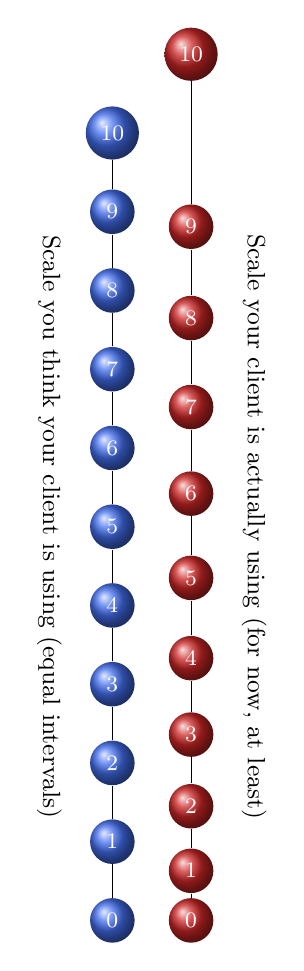
\begin{tikzpicture}[scale=1]
\definecolor{firebrick2}{RGB}{205,38,38};
\definecolor{royalblue2}{RGB}{67,110,238};
\pgfmathtruncatemacro{\T}{10}
\tikzstyle{every node}=[draw=none,shape=circle,ball color=royalblue2,minimum size=5.5mm, white];
\foreach \n in {0,...,\T} 
\node (\n) at (0,\n) {\footnotesize{\n}};
\foreach \n [remember=\n as \lastn (initially 0)] in {0,...,\T} 
\draw (\lastn) -- (\n);
\tikzstyle{every node}=[draw=none,shape=circle,ball color=firebrick2,minimum size=5.5mm, white];
\def\myarray{{0,0.63,1.45,2.36,3.33,4.35,5.42,6.52,7.65,8.81,11}};
\foreach \x [count=\xi] in {0,...,10} 
\node (\x) at (1,\myarray[\x]) {\footnotesize{\x}};
\foreach \x [remember=\x as \lastx (initially 0)] in {0,...,\T} 
\draw (\lastx) -- (\x);
\tikzstyle{every node}=[rotate=-90];
\node at (-0.8,5) {\small{Scale you think your client is using (equal intervals)}};
\node at (1.8,5) {\small{Scale your client is actually using (for now, at least)}};
\end{tikzpicture} 
\end{document}